\documentclass{amsart}

\usepackage{graphicx}



\title{The Iterative Fiedler vs. the generalized Fiedler clustering methods}
\author{Keivan Hassani Monfared}
\address{k1monfared@gmail.com}

\begin{document}
\maketitle

\begin{abstract}
	Here we explore the difference between two clustering methods of simple graphs using an eigenvector corresponding to the second smallest eigenvalue of the Laplacian of the graph: the iterative method and the generalized one. The numerical experiments show that the iterative method on average performs better in most cases.
\end{abstract}

\section{Introduction}
	The \textbf{iterative Fiedler clustering method} is as follows:
	\begin{enumerate}
		\item Start with all the vertices in one cluster.
		\item For each cluster:
		\begin{enumerate}
			\item consider this cluster as a standalone graph,
			\item divide the cluster into two clusters by separating the positive and negative components of the second smallest eigenvector of the Laplacian.
		\end{enumerate}
		\item Repeat until each cluster consists of only one vertex.
	\end{enumerate}
	
	One consideration with this method is which cluster shall be separated first. To address this, we compute the normalized algebraic connectivity of each cluster and choose the one with the lowest algebraic connectivity to be separated first.
	
	Another consideration with this method is that for subgraphs the second smallest eigenvector of the Laplacian does not take into account the external forces that pull vertices together (push away from each other, in the case of negative edges), that is, it ignores the edges outside the subgraph. 
	
	One suggested workaround for both of these concerns is to use more eigenvectors of the Laplacian of the whole graph to cluster in one step. This gives rise to a new method for clustering. 
	
	The \textbf{generalized Fiedler clustering method} is as follows:
	\begin{enumerate}
		\item Compute $k$ largest eigenvectors of the Laplacian of the graph ($k \leq \log_2(n)$, where $n$ is the number of vertices of the graph).
		\item Put the vertices with the same sign patterns in the same cluster.
	\end{enumerate}
	
	Two families of graph were generated; first, graphs with $4$ clusters on $78$ vertices of comparable sizes $20$, $15$, $25$, and $18$; second, graphs with $4$ clusters of sizes $100$, $12$, $8$, and $15$. The density of edges inside each cluster is $90\%$, and we let the density of the edges between clusters to vary from $0\%$ to $99\%$, with increments of $1\%$. For example, and example when the inter density is a $10\%$ is shown in Figure \ref{two_sample_clustered_matrices}.
		
		\begin{figure}[h]
		\begin{center}
			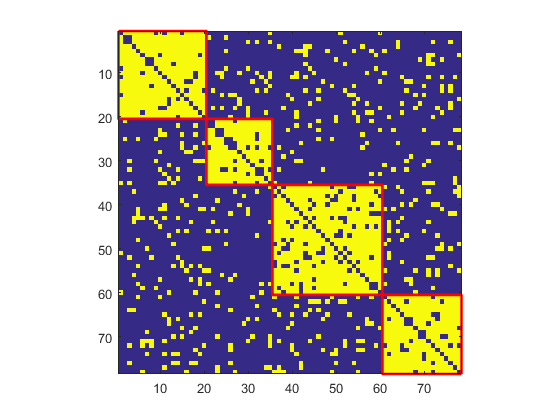
\includegraphics[scale=.4]{90intra10inter_20_15_25_18}
			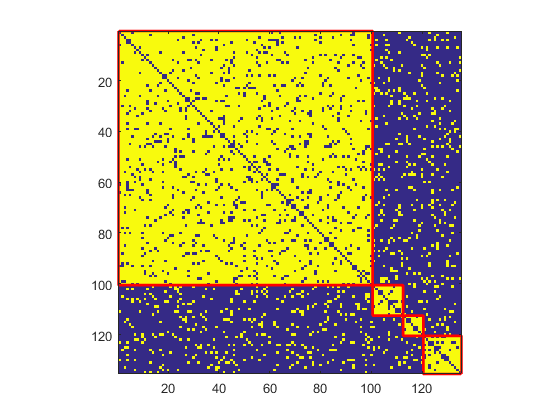
\includegraphics[scale=.4]{90intra10inter_100_12_8_15}
			\caption{The adjacency matrices of two graphs with four clusters (Left:) of comparable sizes, and (Right:) of non-comparable sizes. Both graphs have $90\%$ intra density and $10\%$ inter density.}
			\label{two_sample_clustered_matrices}
		\end{center}
		\end{figure}
		
\newpage		
	\section{Methods}
		For each density of inter edges, we generated $1000$ random graphs, and applied two methods of clustering on them. The adjusted Rand index (ARI) against our known clustering, and the Girvan-Newman modularity (GNM) for each clustering was computed and the average of them is recorded.
			

\newpage	
	\section{Results}
	
		\subsection{Clusters with almost equal sizes}
			Since the meaning of cluster fades away as the density of inter edges increases, we have included figures of a range of densities for better intuition in Figure \ref{four_comparable_clusters_samples}.
			
			\begin{figure}[h]
			\begin{center}
				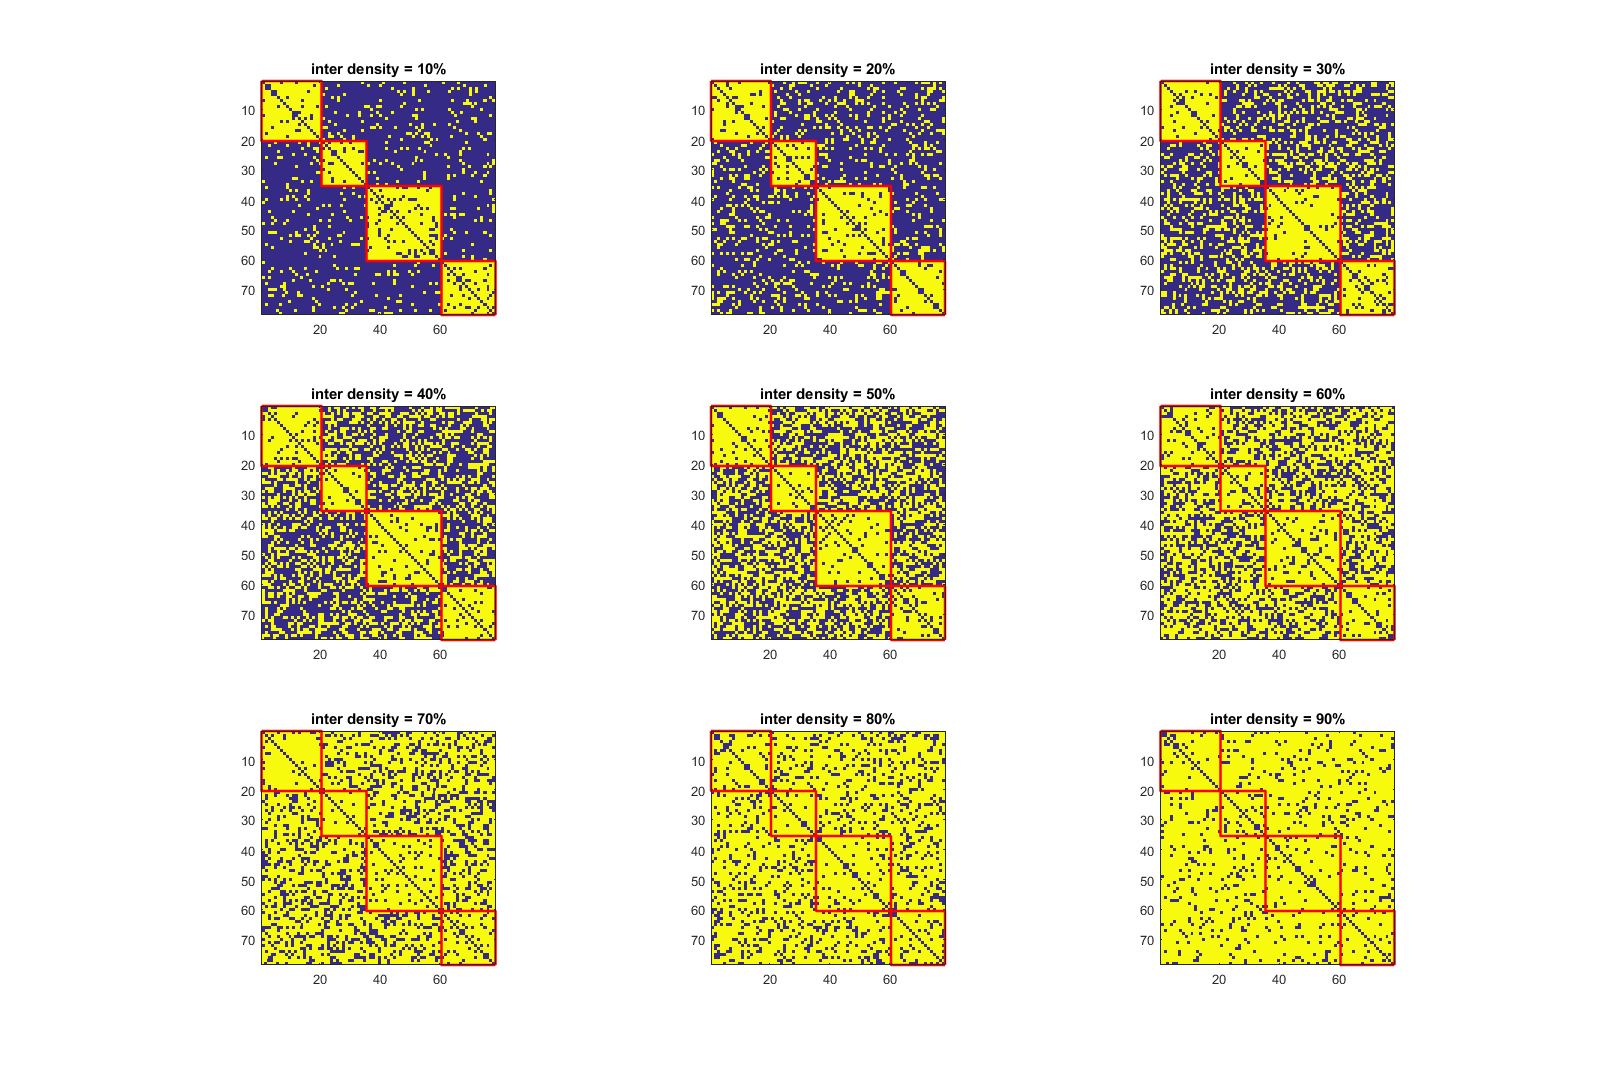
\includegraphics[width = \linewidth, trim = 150 70 150 30, clip]{four_comparable_clusters_samples}
				\caption{Sample graphs with four clusters of comparable sizes.}
				\label{four_comparable_clusters_samples}
			\end{center}
			\end{figure}
			
			And here are the results:
			
			\begin{figure}[h]
			\begin{center}
				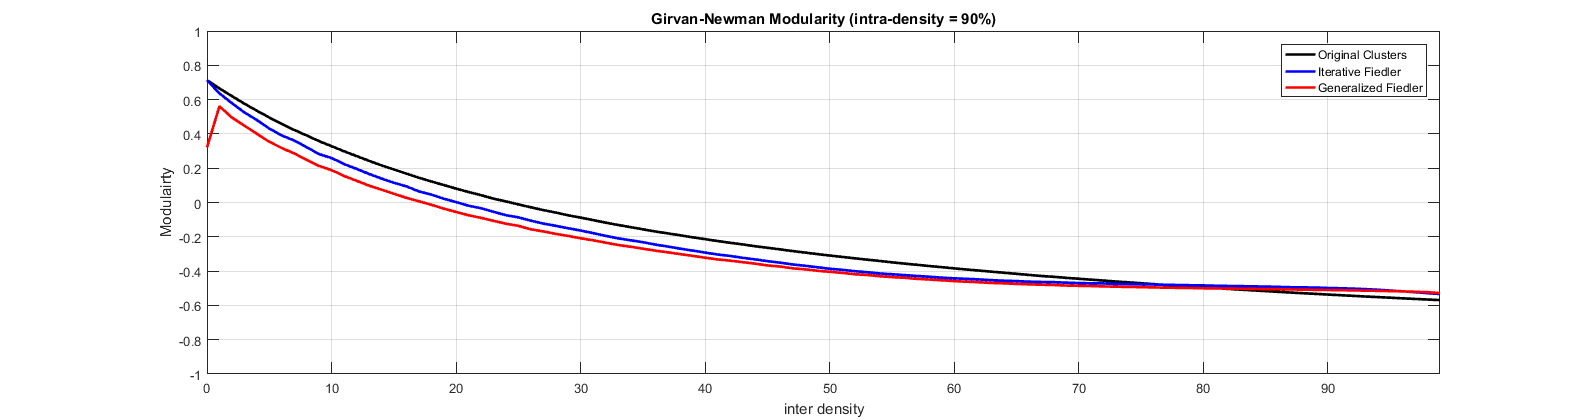
\includegraphics[width = \linewidth, trim = 70 0 70 10, clip]{four_comparable_clusters_modularity}
				\caption{Averages of Girvan-Newman modularity of graphs with four clusters of comparable sizes for each inter density for $1000$ runs each.}
				\label{four_comparable_clusters_GNM}
			\end{center}
			\end{figure}
		
			\begin{figure}[h]
			\begin{center}
				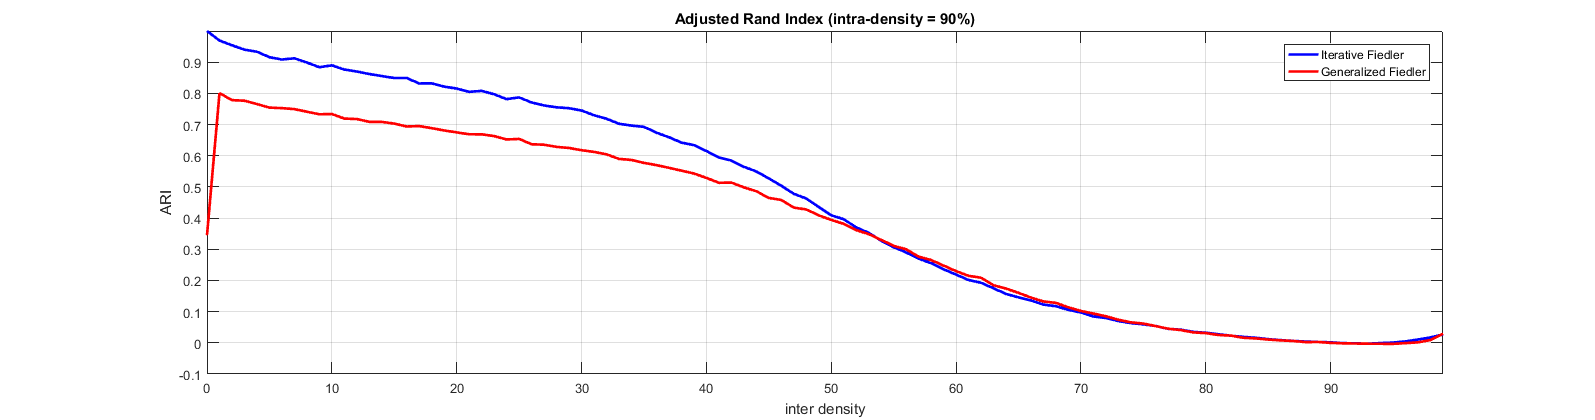
\includegraphics[width = \linewidth, trim = 70 0 70 10, clip]{four_comparable_clusters_ari}
				\caption{Averages of adjusted Rand index of graphs with four clusters of comparable sizes for each inter density for $1000$ runs each.}
				\label{four_comparable_clusters_ARI}
			\end{center}
			\end{figure}
	
		\subsection{Clusters with sizes far away from each other}
			When the sizes of clusters are different from each other however, the methods do not behave in the same way. In particular, the modularity cannot reach the theoretical maximum and overall stays low.
			\begin{figure}[h]
			\begin{center}
				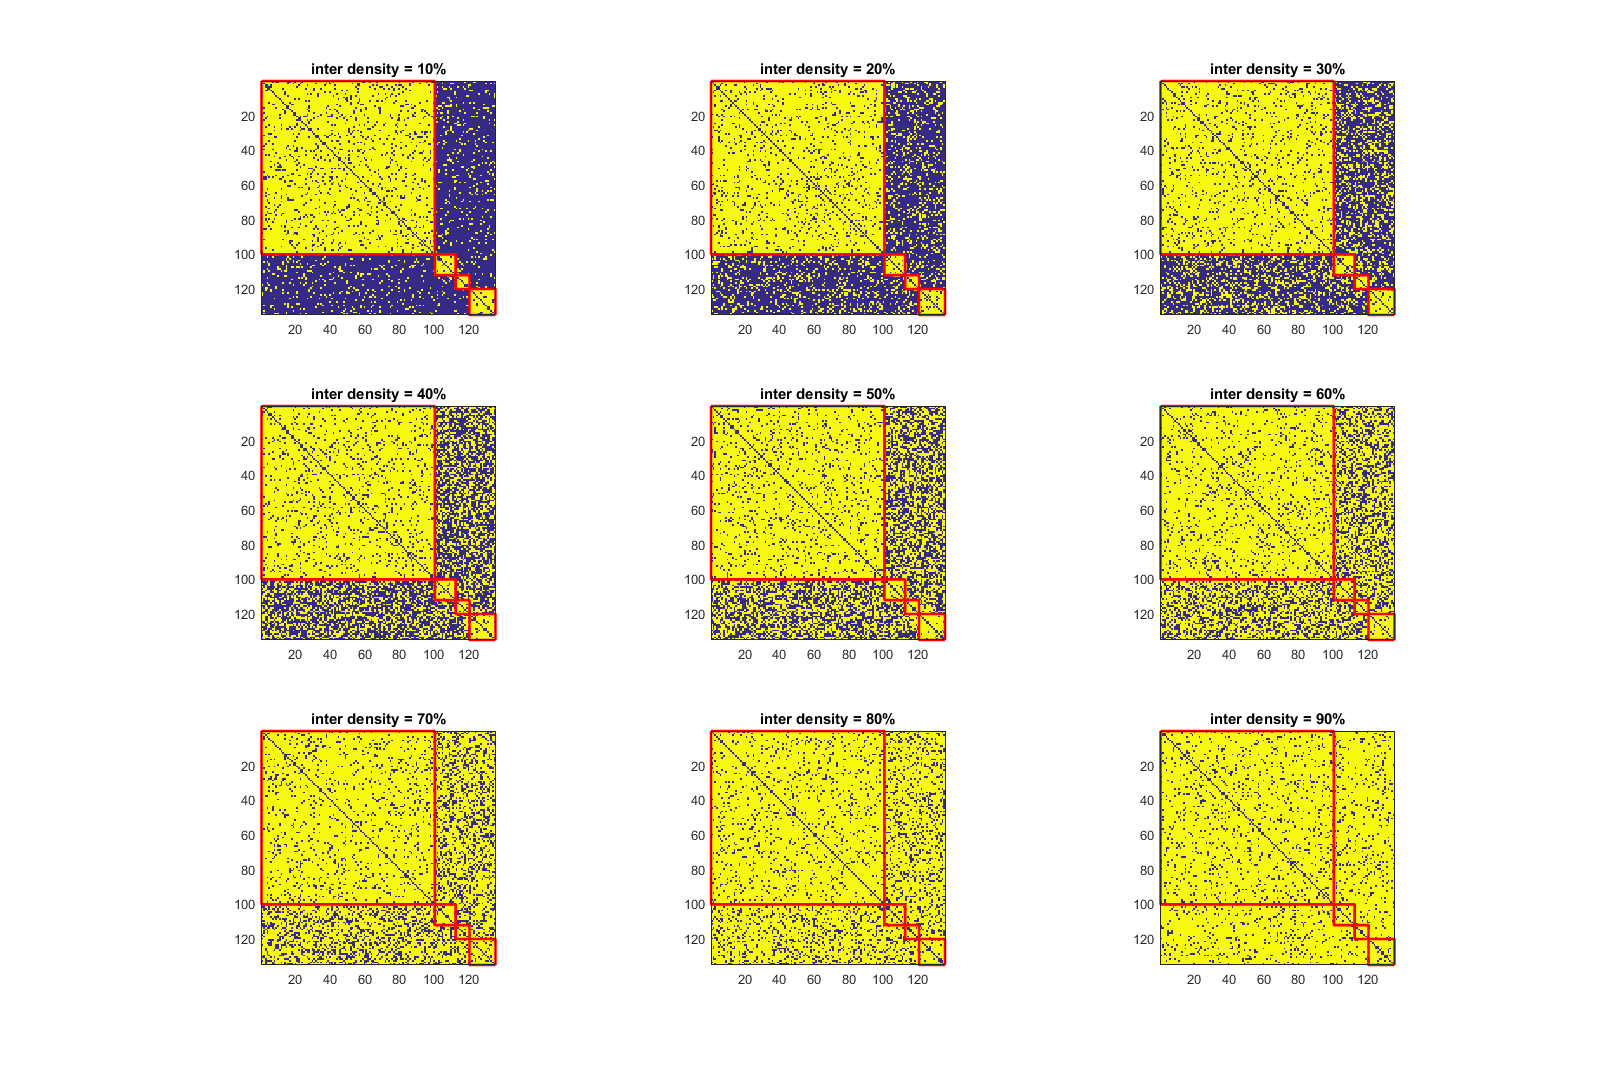
\includegraphics[width = \linewidth, trim = 150 70 150 30, clip]{four_faraway_clusters_samples}
				\caption{Sample graphs with four clusters of far away sizes.}
				\label{four_faraway_clusters_samples}
			\end{center}
			\end{figure}
			
			And here are the results:
			
			\begin{figure}[h]
			\begin{center}
				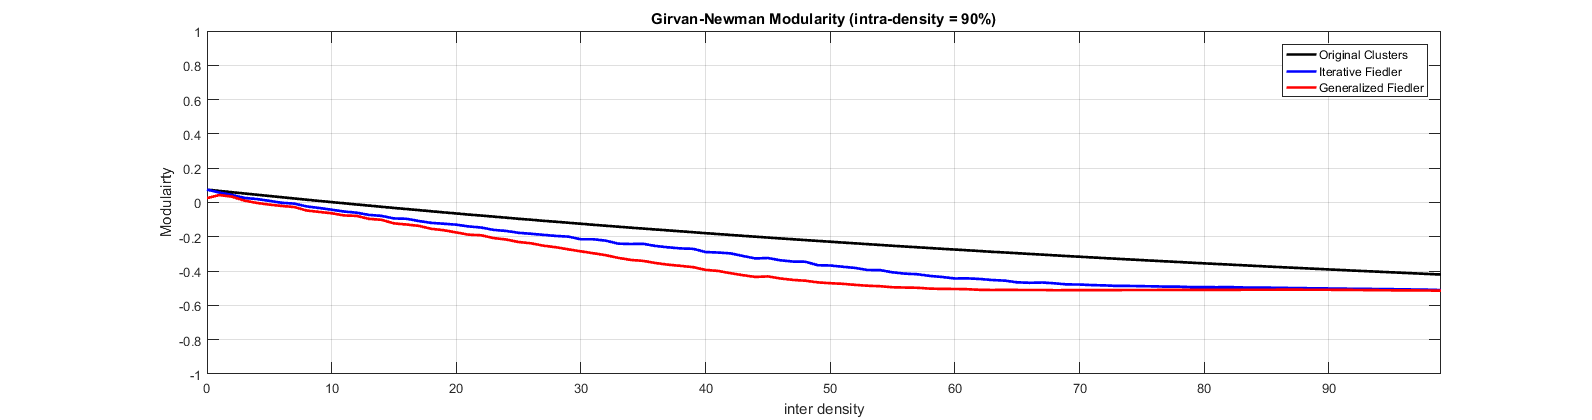
\includegraphics[width = \linewidth, trim = 70 0 70 10, clip]{four_faraway_clusters_modularity}
				\caption{Averages of Girvan-Newman modularity of graphs with four clusters of far away sizes for each inter density for $1000$ runs each.}
				\label{four_faraway_clusters_GNM}
			\end{center}
			\end{figure}
		
			\begin{figure}[h]
			\begin{center}
				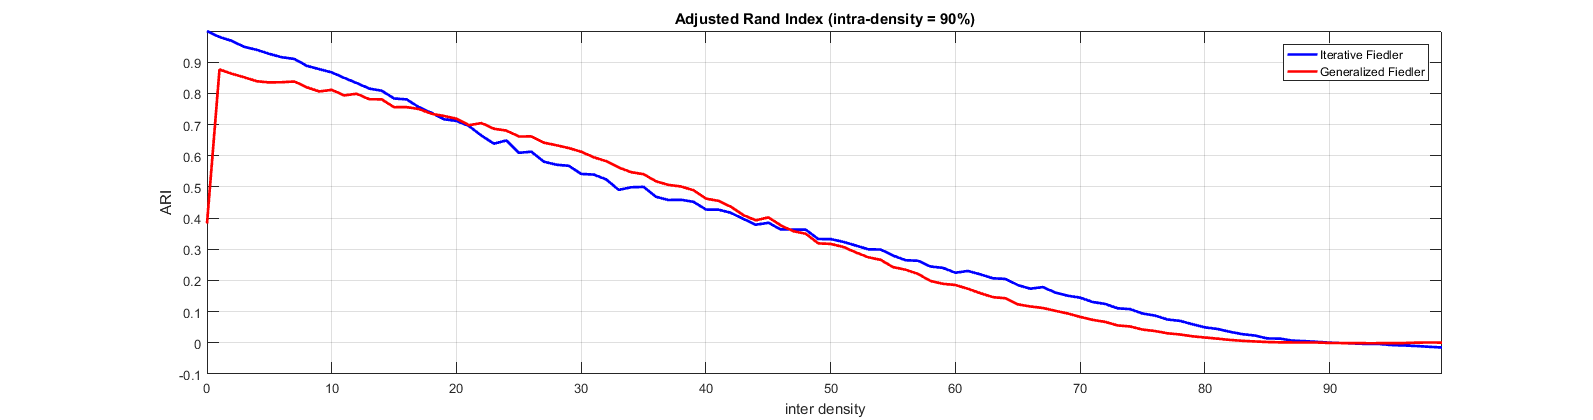
\includegraphics[width = \linewidth, trim = 70 0 70 10, clip]{four_faraway_clusters_ari}
				\caption{Averages of adjusted Rand index of graphs with four clusters of far away sizes for each inter density for $1000$ runs each.}
				\label{four_faraway_clusters_ARI}
			\end{center}
			\end{figure}
			
\begin{thebibliography}{9}
	\bibitem{f73} M. Fiedler. ``Algebraic connectivity of Graphs'', Czechoslovak Mathematical Journal 23(98) (1973), 298--305.
	
	\bibitem{f75} Keivan Hassani Monfared, Kris Vasudevan, Jordan S. Farrell, G. Campbell Teskey, ``Community structure detection and evaluation during the pre- and post-ictal hippocampal depth recordings'',	arXiv:1804.01568 [cs.SI].
\end{thebibliography}
\end{document}